\pr Fieles a la recomendación del Salvador y siguiendo su divina enseñanza, nos atrevemos a decir:

\begin{center}
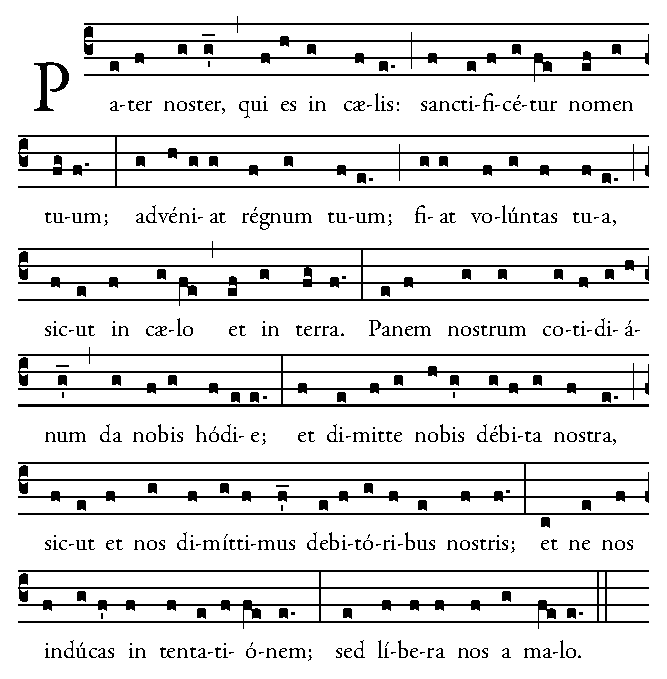
\includegraphics[width=.9\textwidth]{src/ordinario/pater.eps}
\end{center}

\be Padre nuestro, que estás en el cielo,\redast santificado sea tu Nombre;\redast venga a nosotros tu reino;\redast hágase tu voluntad en la tierra como en el cielo.\redast Danos hoy nuestro pan de cada día;\redast perdona nuestras ofensas,\redast como también nosotros perdonamos\redast a los que nos ofenden;\redast no nos dejes caer en la tentación,\redast y líbranos del mal.

\pr Líbranos de todos los males, Señor, y concédenos la paz en nuestros días, para que, ayudados por tu misericordia, vivamos siempre libres de pecado y protegidos de toda perturbación, mientras esperamos la gloriosa venida de nuestro Salvador Jesucristo.

\be Tuyo es el reino, tuyo el poder y la gloria, por siempre, Señor.

\pr Señor Jesucristo, que dijiste a tus apóstoles: “La paz os dejo, mi paz os doy”; no tengas en cuenta nuestros pecados, sino la fe de tu Iglesia y, conforme a tu palabra, concédele la paz y la unidad. Tú que vives y reinas por los siglos de los siglos.

\be Amén.

\pr La paz del Señor esté siempre con vosotros.

\be Y con tu espíritu.

\pr Daos fraternalmente la paz.

\begin{center}

\includegraphics[width=.9\textwidth]{src/ordinario/agnus.eps}
\end{center}

\be Cordero de Dios, que quitas el pecado del mundo,\redast ten piedad de nosotros.
\be Cordero de Dios, que quitas el pecado del mundo,\redast ten piedad de nosotros.
\be Cordero de Dios, que quitas el pecado del mundo,\redast danos la paz.

\pr Éste es el Cordero de Dios, que quita el pecado del mundo. Dichosos los invitados a la cena del Señor.

\be Señor, no soy digno de que entres en mi casa, pero una palabra tuya bastará para sanarme.

\pr Oremos.

\pr Te rogamos, Señor, que, purificados ya de nuestras pasadas culpas, la participación en este sacramento de tu Hijo nos transforme en hombres nuevos. Por Jesucristo nuestro Señor.

\be Amén.